\section{Resultados}
    En la presenta sección se exponen los resultados más relevantes obtenidos de 
    aplicar los filtros de recorte sobre las imágenes del dataset dado para el proyecto. 
    Se adiciona algunas características del resultado final y para observar de 
    mejor manera las imágenes referirse a la libreta de Jupyter del proyecto (\href{https://github.com/alexisuaguilaru/ProcDigImg/blob/main/Proy04/proyecto.ipynb}{proyecto.ipynb}) 
    que además sirve de bitácora para los experimentos realizados (definición de los filtros).

    \subsection{Imagen 1}
        Aunque cuenta con destellos notorios cercanos al centro del dominio, nos encontramos 
        con que también aparecen líneas que pueden ser difíciles de eliminar con filtros 
        de recorte, haciendo que en la imagen resultante aún conserve parte de ese ruido 
        periódico en forma de líneas diagonales. 

        \begin{figure}[H]
            \centering
            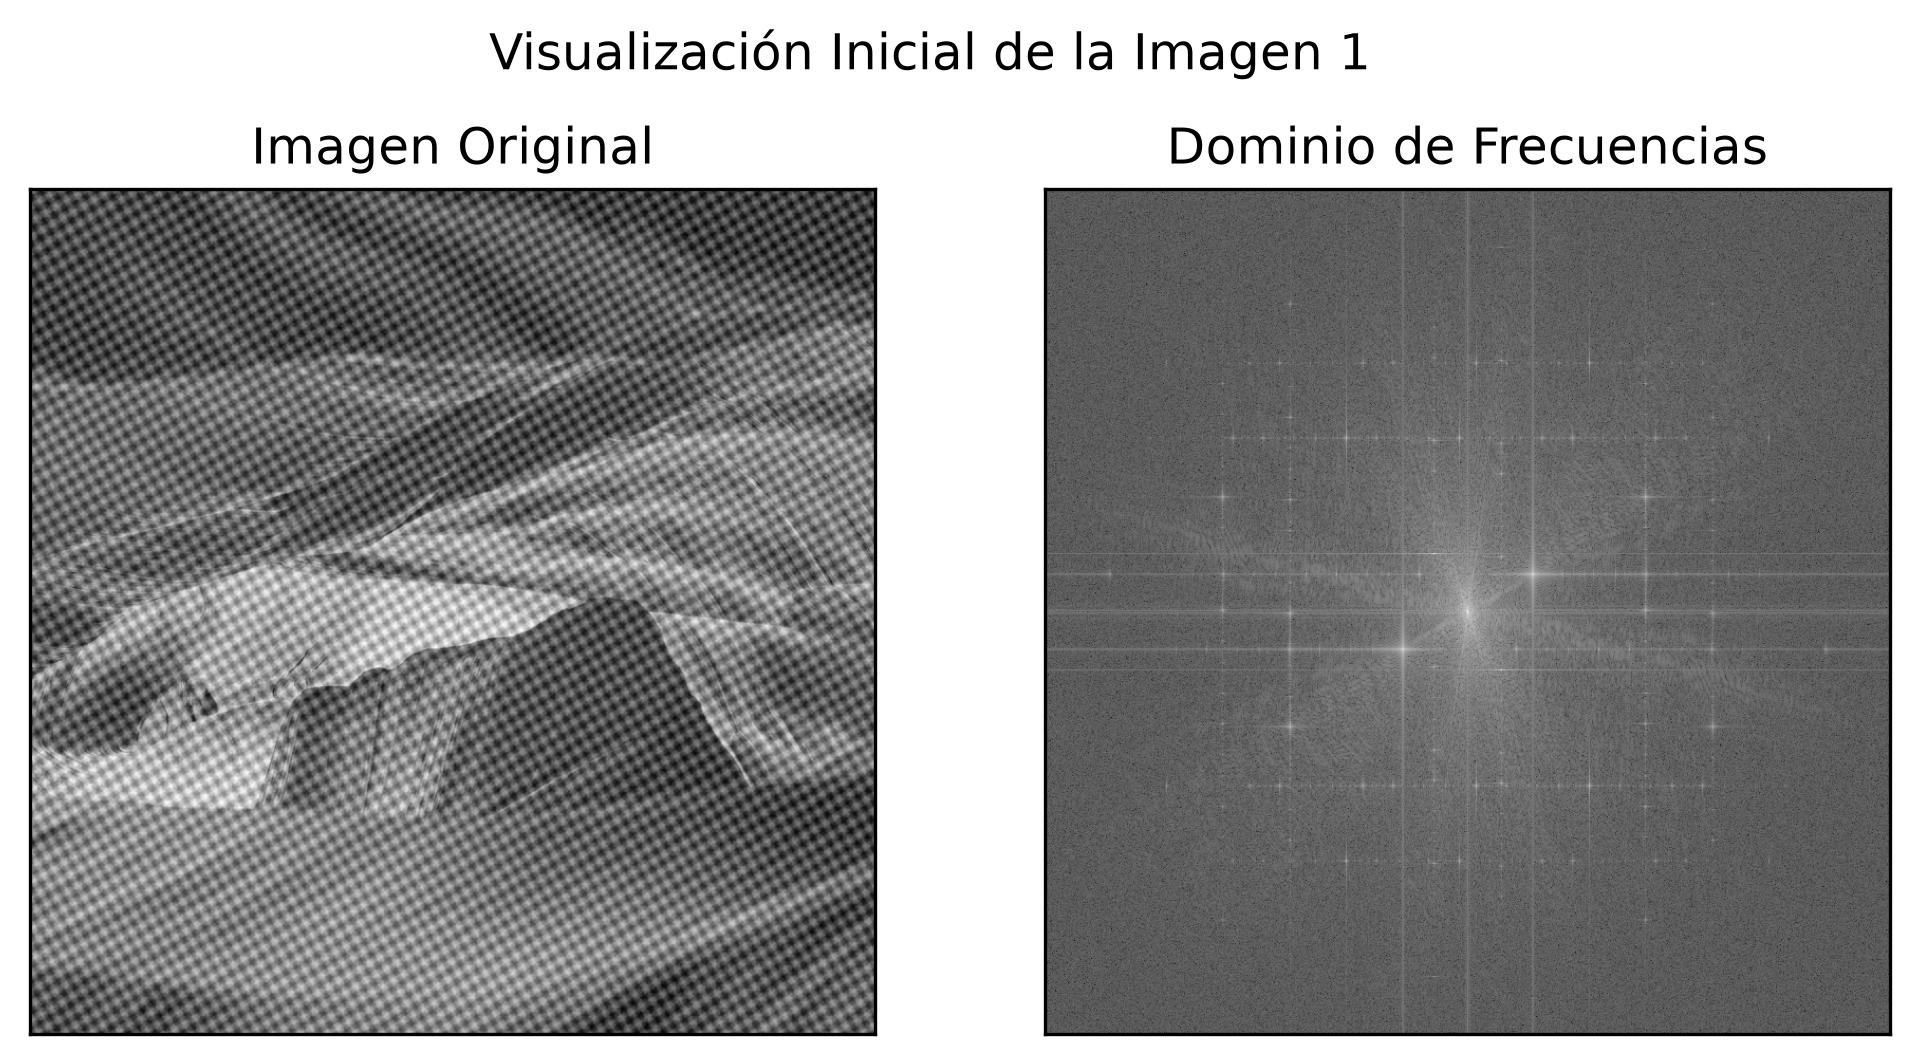
\includegraphics[width=0.65\textwidth]{../results/img_1_initial.jpg}
            \caption{Imagen 1 con ruido periódico.}
        \end{figure}

        \begin{figure}[H]
            \centering
            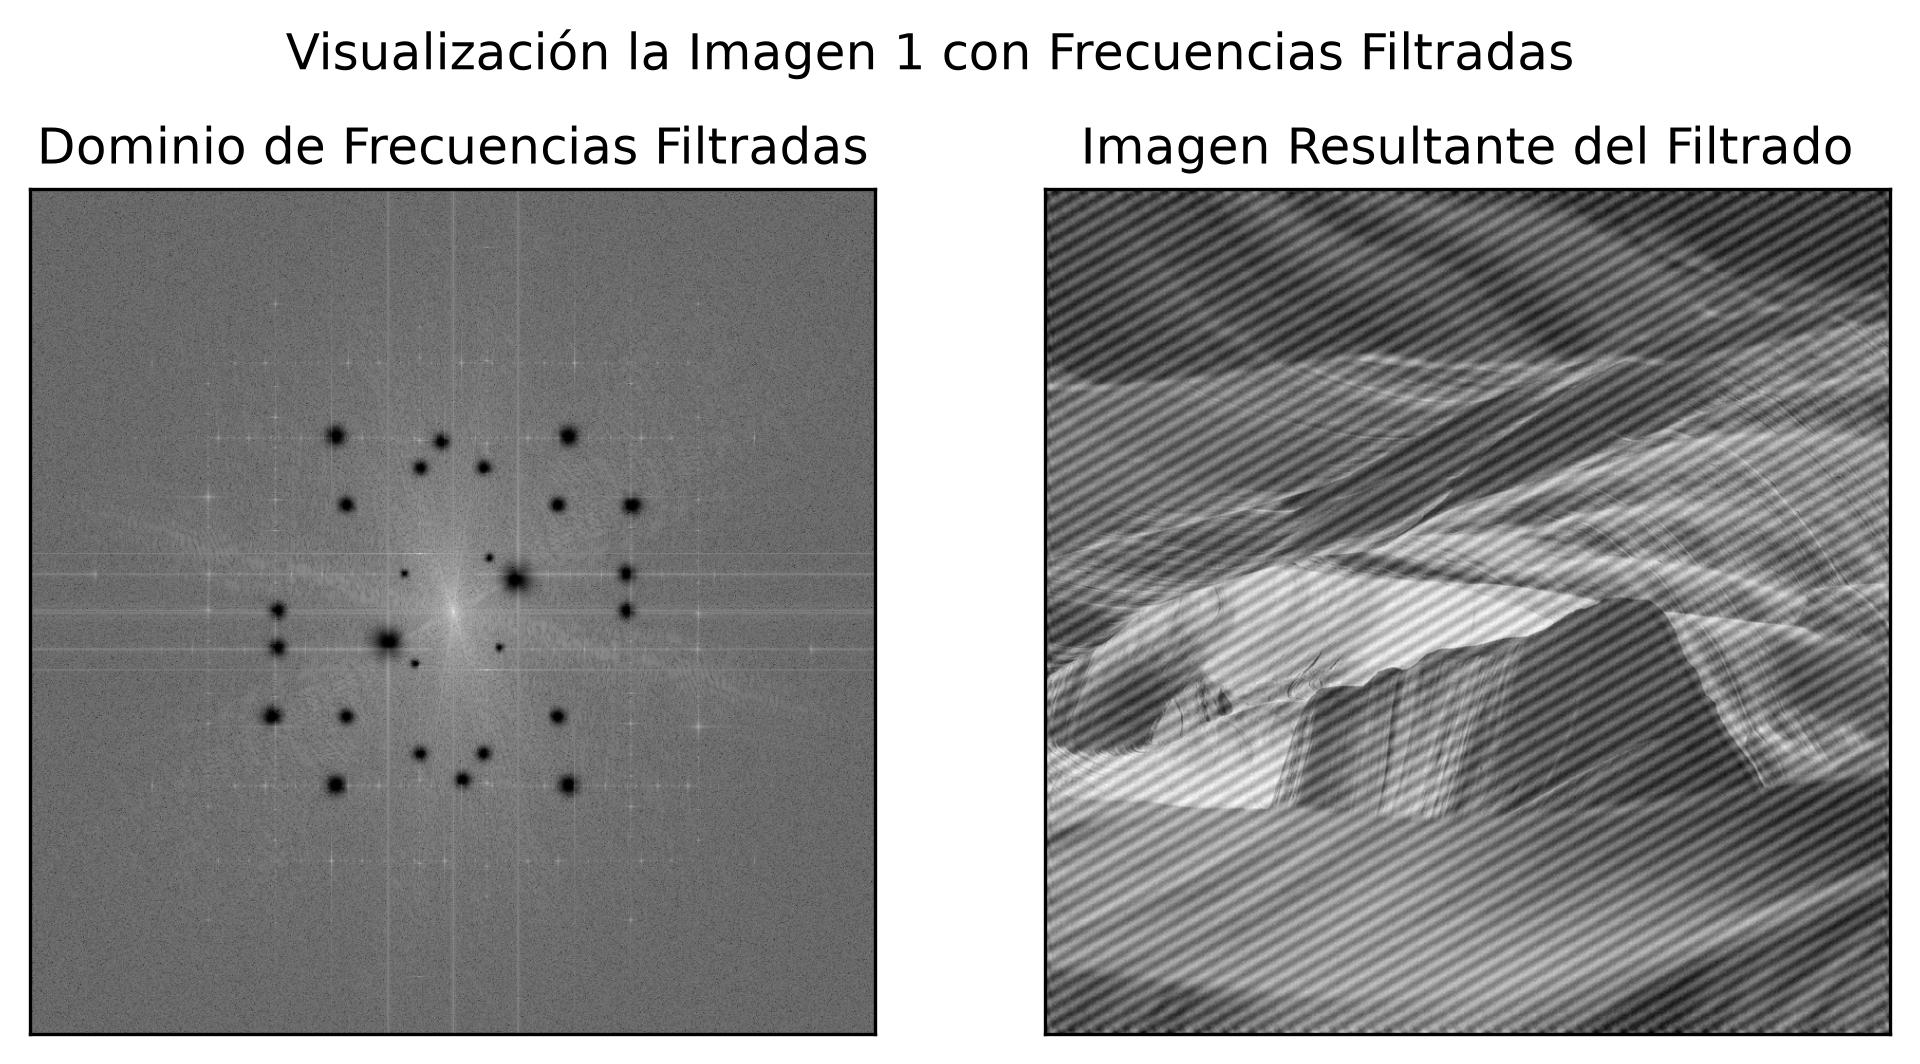
\includegraphics[width=0.65\textwidth]{../results/img_1_final.jpg}
            \caption{Imagen 1 después del filtrado de frecuencias.}
        \end{figure}

    \subsection{Imagen 2}
        Al observar el dominio de frecuencias notamos que presenta destellos 
        dominantes que al ser eliminados revelamos de forma significativa la 
        imagen oculta por el ruido. Pero aún así se conserva algunas líneas 
        diagonales en los bordes, esto por la presencia de líneas blancas en el espectro.

        \begin{figure}[H]
            \centering
            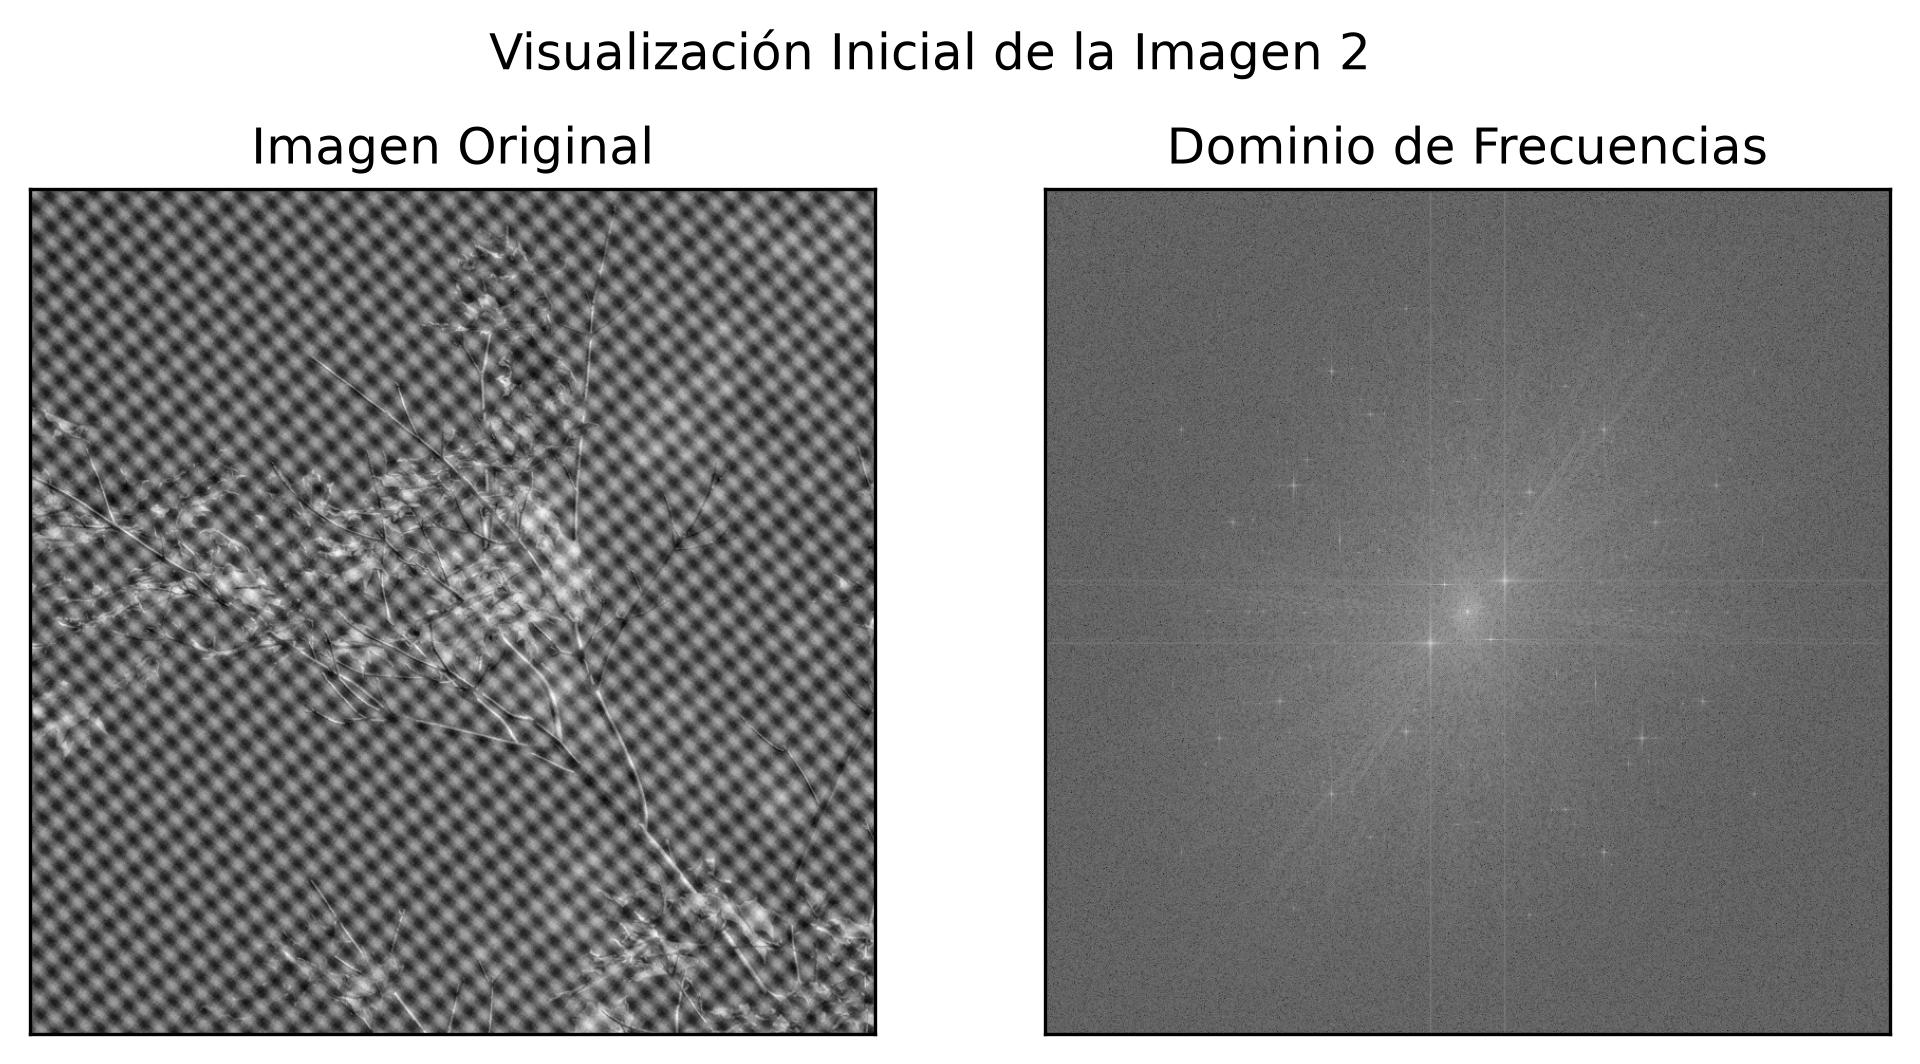
\includegraphics[width=0.65\textwidth]{../results/img_2_initial.jpg}
            \caption{Imagen 2 con ruido periódico.}
        \end{figure}

        \begin{figure}[H]
            \centering
            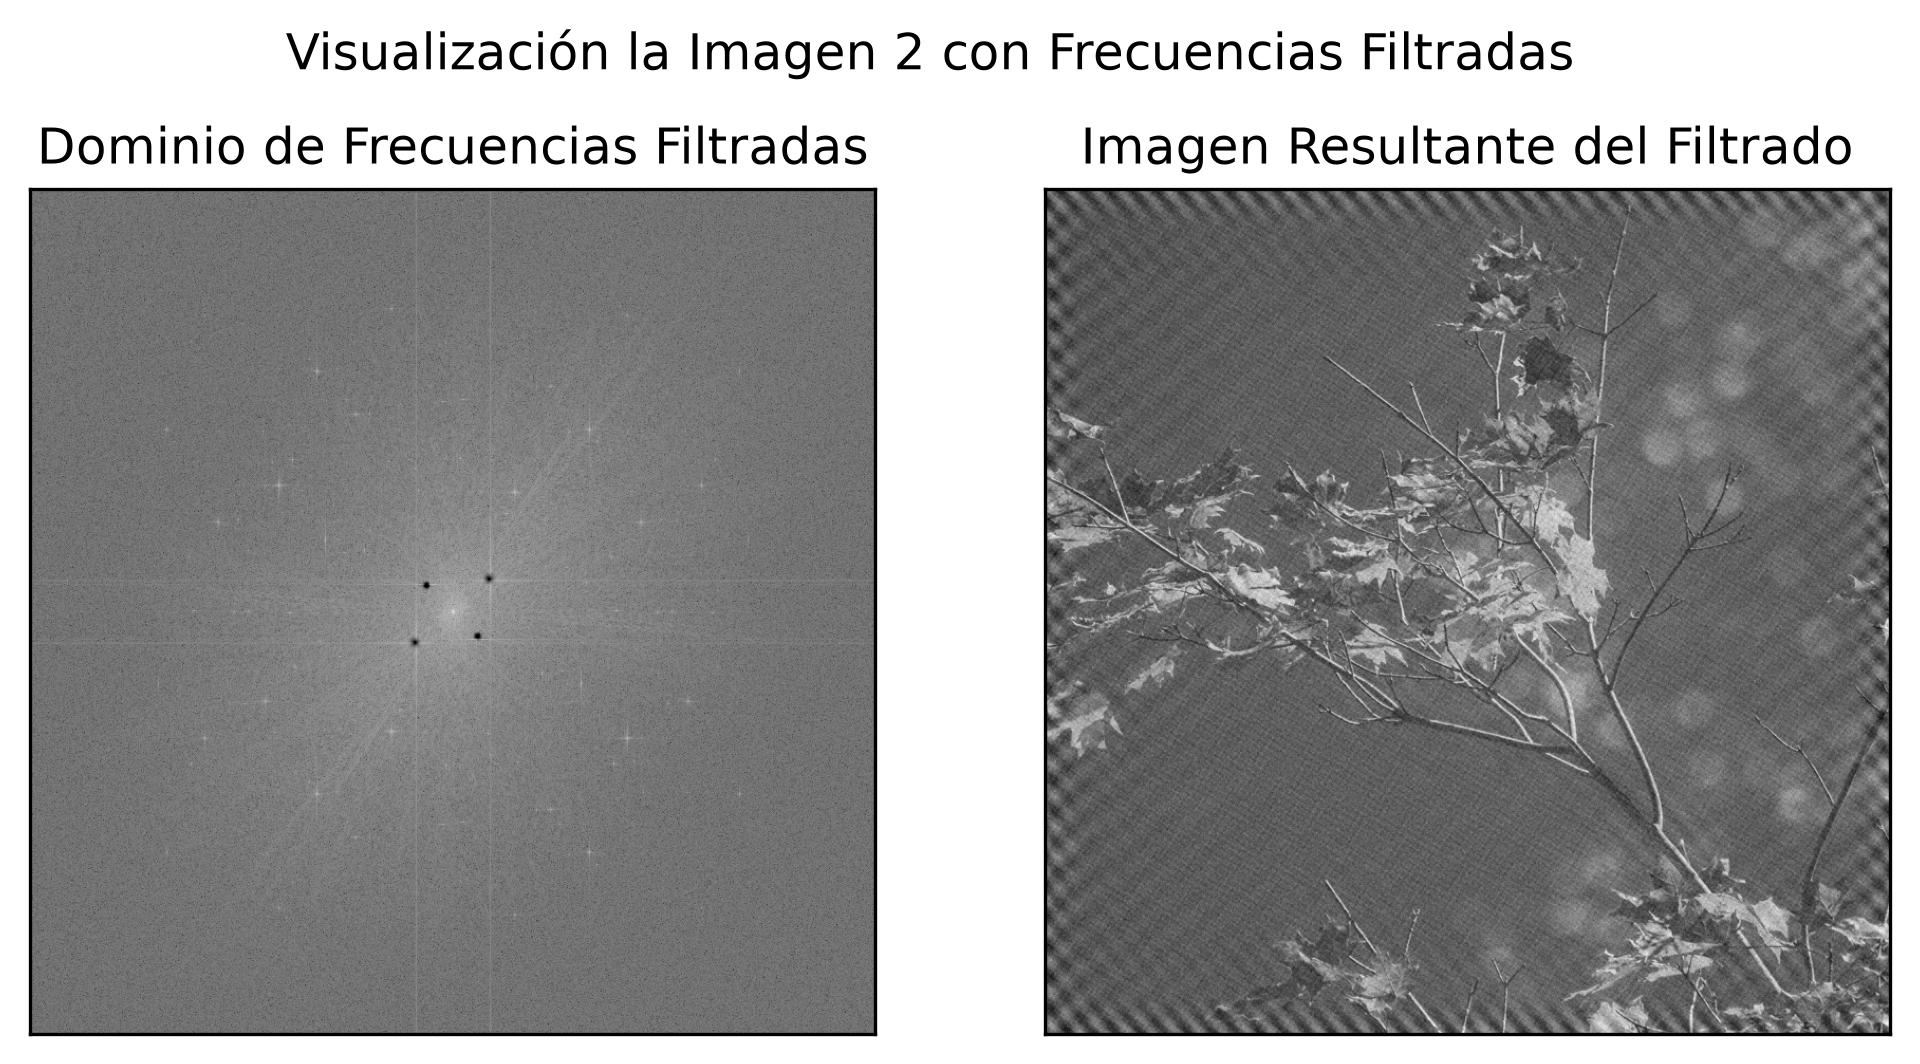
\includegraphics[width=0.65\textwidth]{../results/img_2_final.jpg}
            \caption{Imagen 2 después del filtrado de frecuencias.}
        \end{figure}

    \subsection{Imagen 3}
        Del dominio de frecuencias, podemos notar que existen algunos destellos muy sutiles 
        cerca del centro del espectro, los cuales provocan todo el ruido que notamos 
        en la imagen. Realizando su eliminación de forma precisa, podemos reducir el ruido 
        central de la imagen.

        \begin{figure}[H]
            \centering
            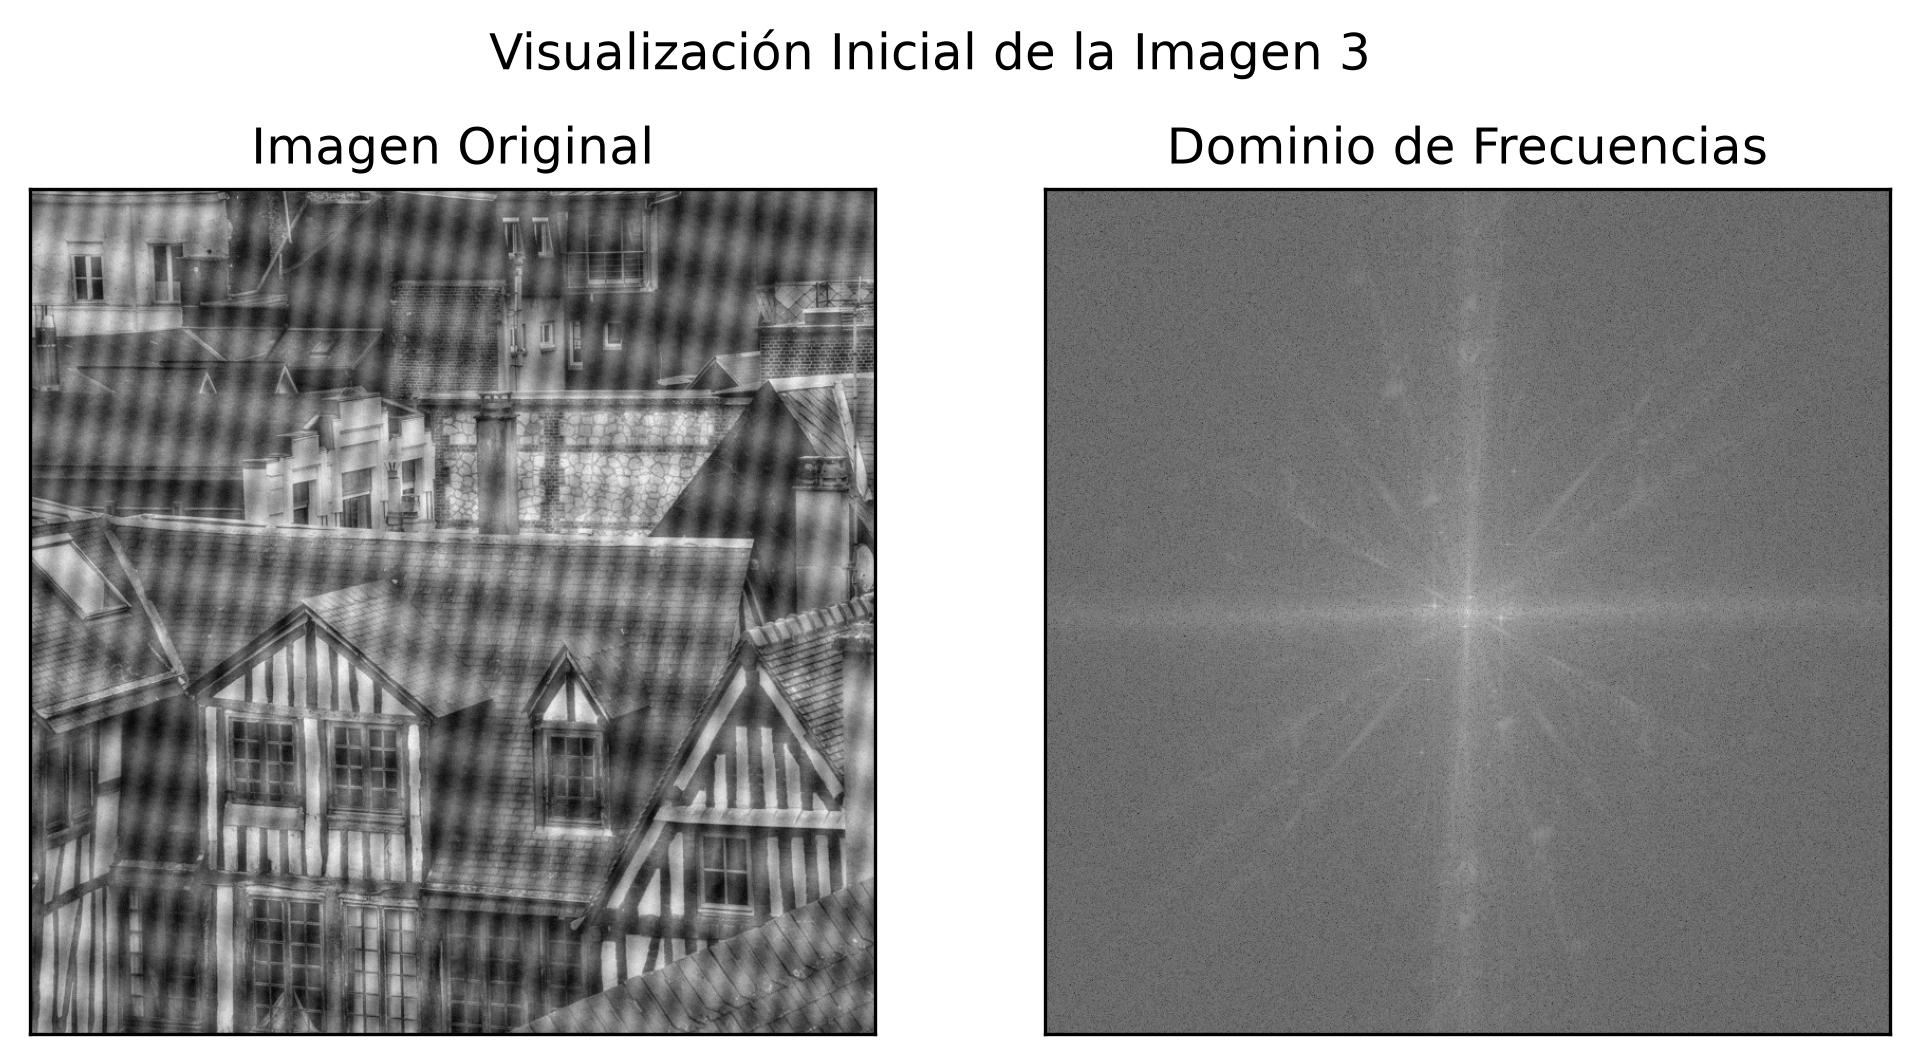
\includegraphics[width=0.65\textwidth]{../results/img_3_initial.jpg}
            \caption{Imagen 3 con ruido periódico.}
        \end{figure}

        \begin{figure}[H]
            \centering
            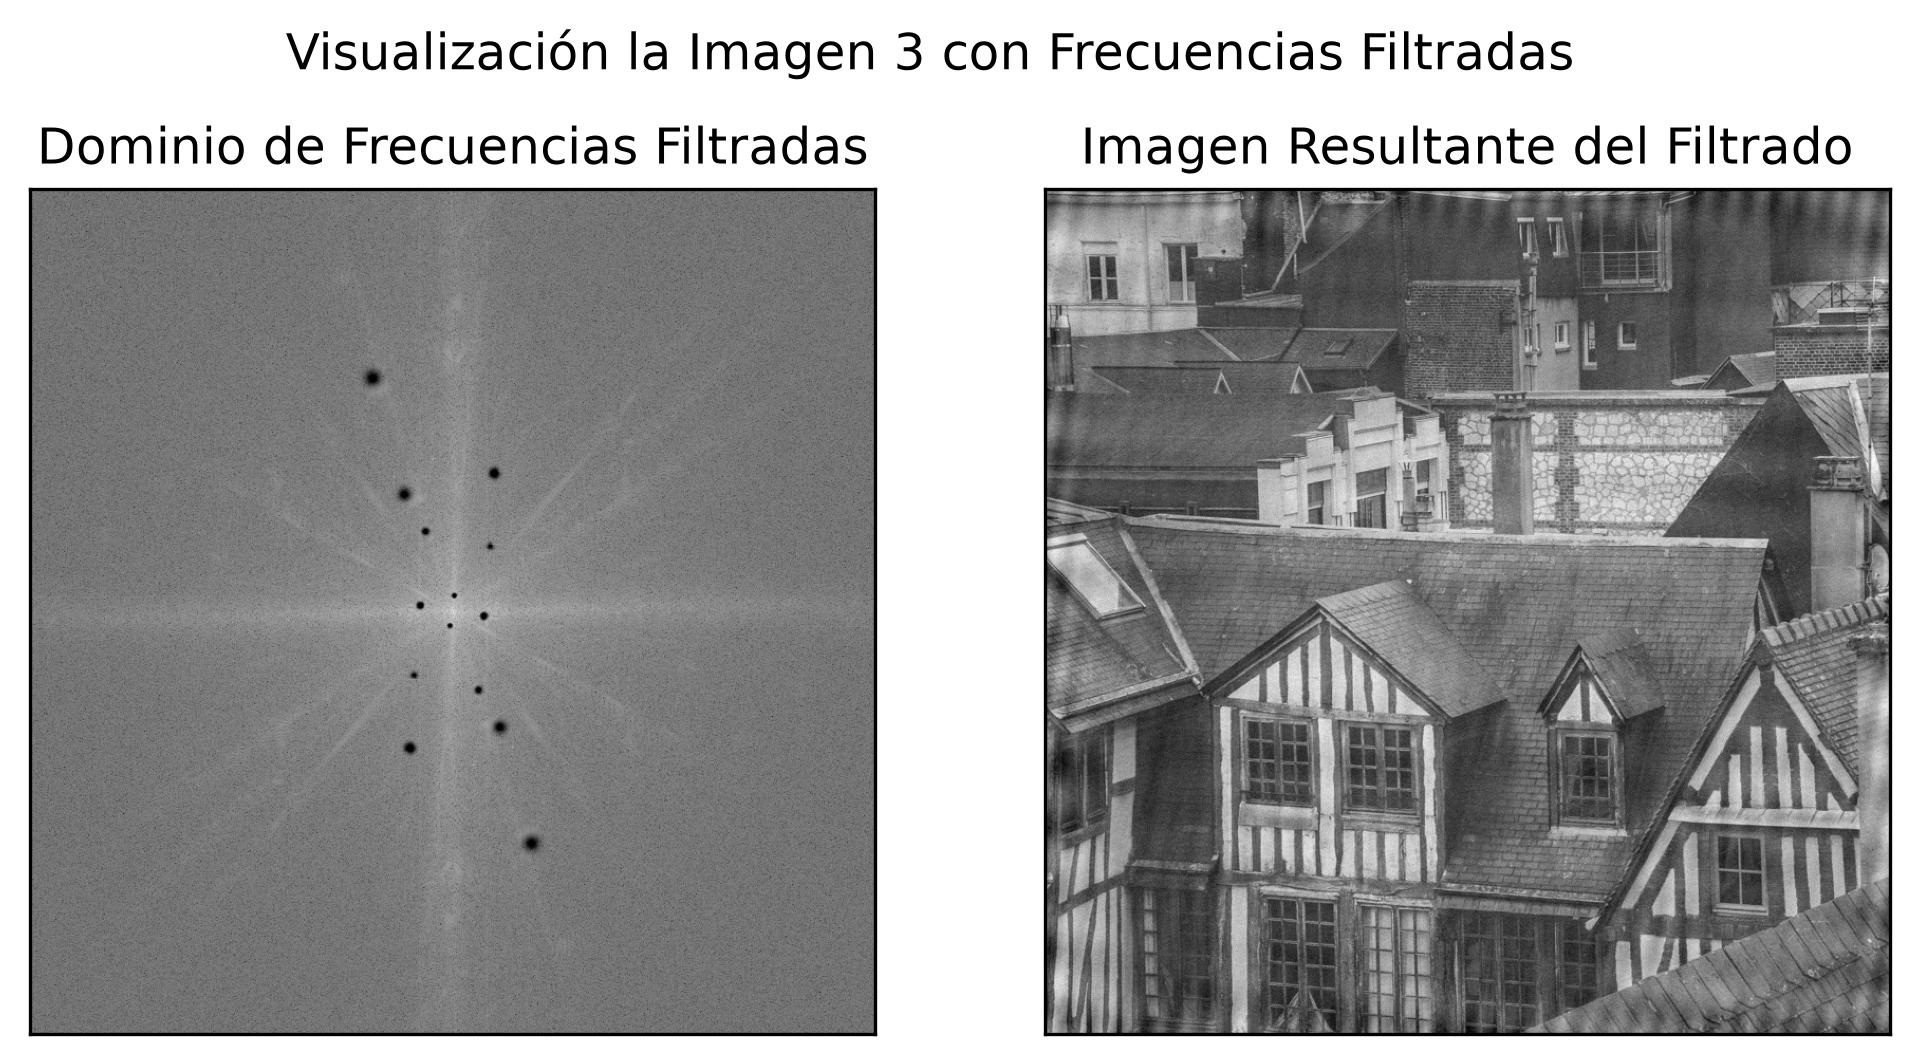
\includegraphics[width=0.65\textwidth]{../results/img_3_final.jpg}
            \caption{Imagen 3 después del filtrado de frecuencias.}
        \end{figure}

    \subsection{Imagen 4}
        Esta imagen se destaca por tener destellos de ruido muy puntuales en el 
        dominio, es decir, no pocas las líneas y todo el ruido es representado 
        de forma puntual, lo cual facilita su mitigación con los filtros adecuados. 
        Lo anterior hace posible observar la imagen sin ruido salvo por los bordes.

        \begin{figure}[H]
            \centering
            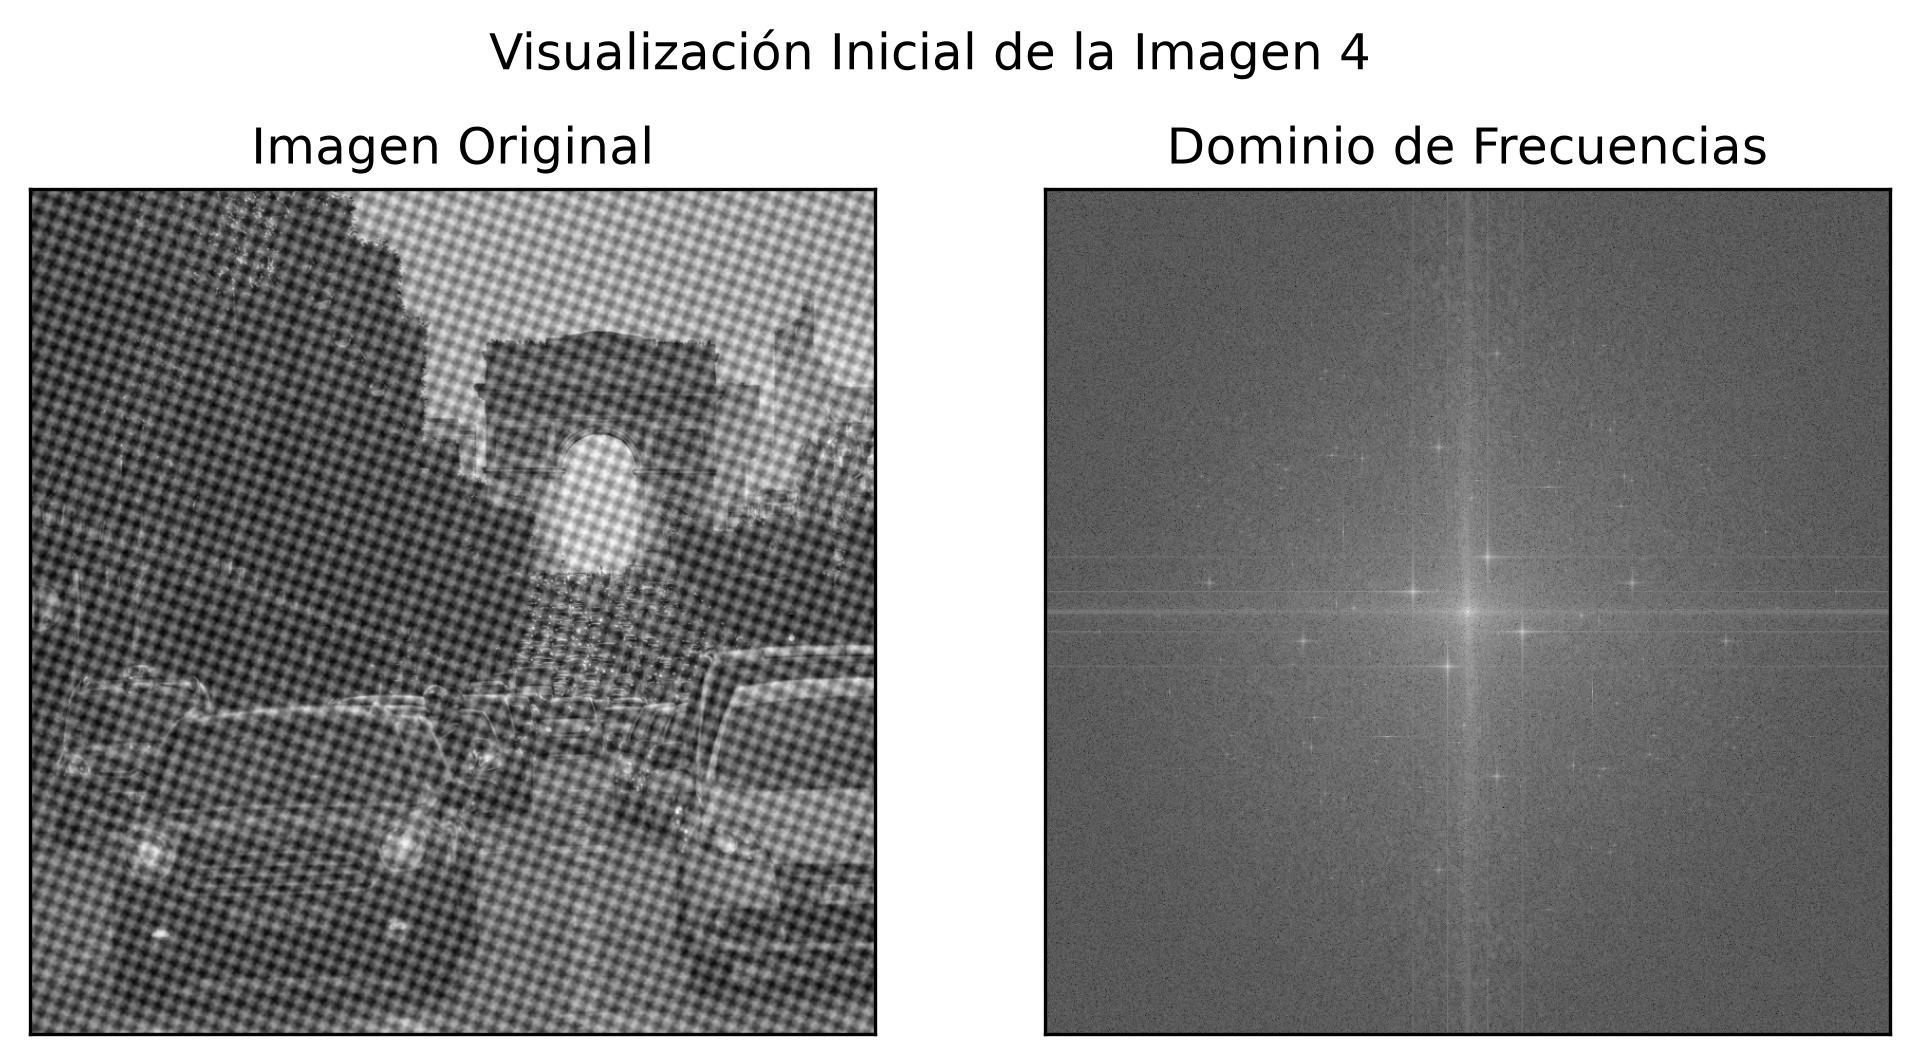
\includegraphics[width=0.65\textwidth]{../results/img_4_initial.jpg}
            \caption{Imagen 4 con ruido periódico.}
        \end{figure}

        \begin{figure}[H]
            \centering
            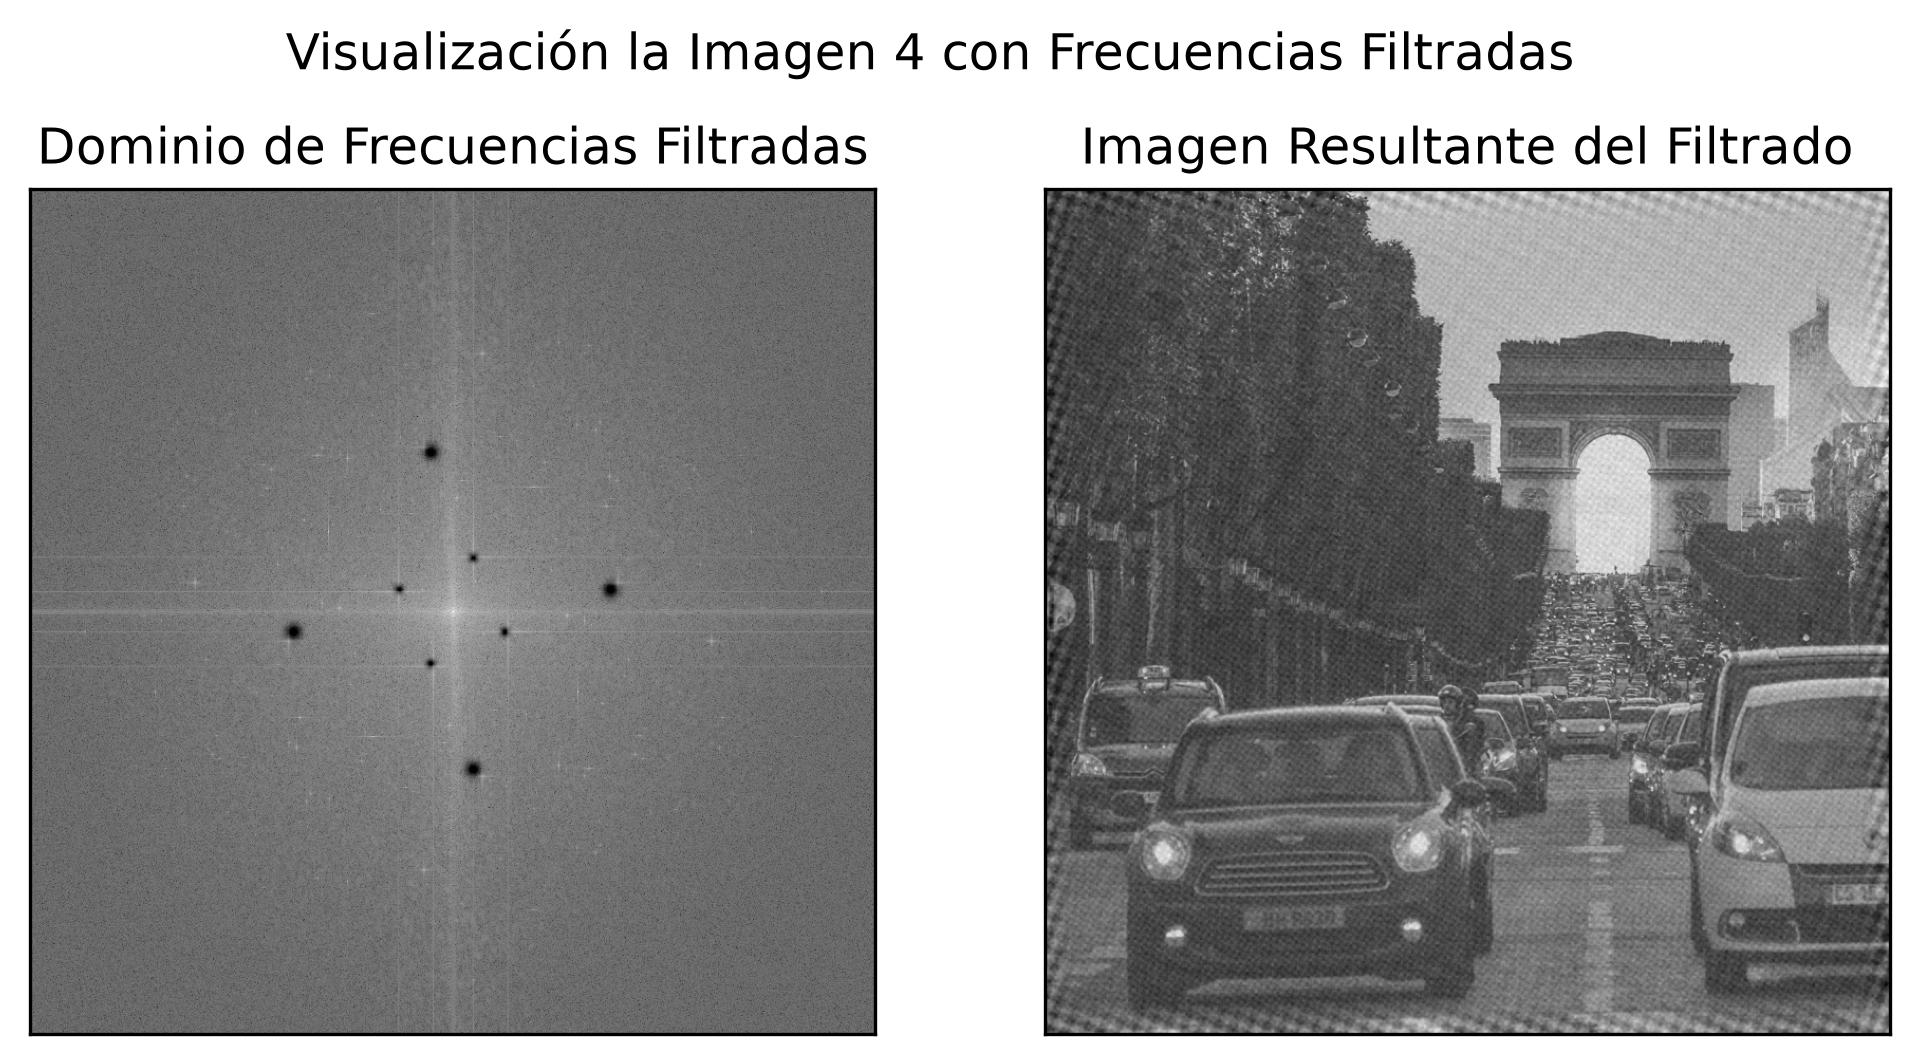
\includegraphics[width=0.65\textwidth]{../results/img_4_final.jpg}
            \caption{Imagen 4 después del filtrado de frecuencias.}
        \end{figure}

    \subsection{Imagen 5}
        Esta es la única imagen que no presenta un ruido pero sí un patrón periódico 
        parte de la imagen, esto hace que su dominio de frecuencias cuente con destellos 
        en forma de patrón. Debido a que el mayor ruido se acumulan como destellos próximos 
        al centro del espectro, si se eliminan algunos de ellos se logra reducir parte 
        del patrón de malla en la imagen, recuperando el elemento detrás de la malla. 

        \begin{figure}[H]
            \centering
            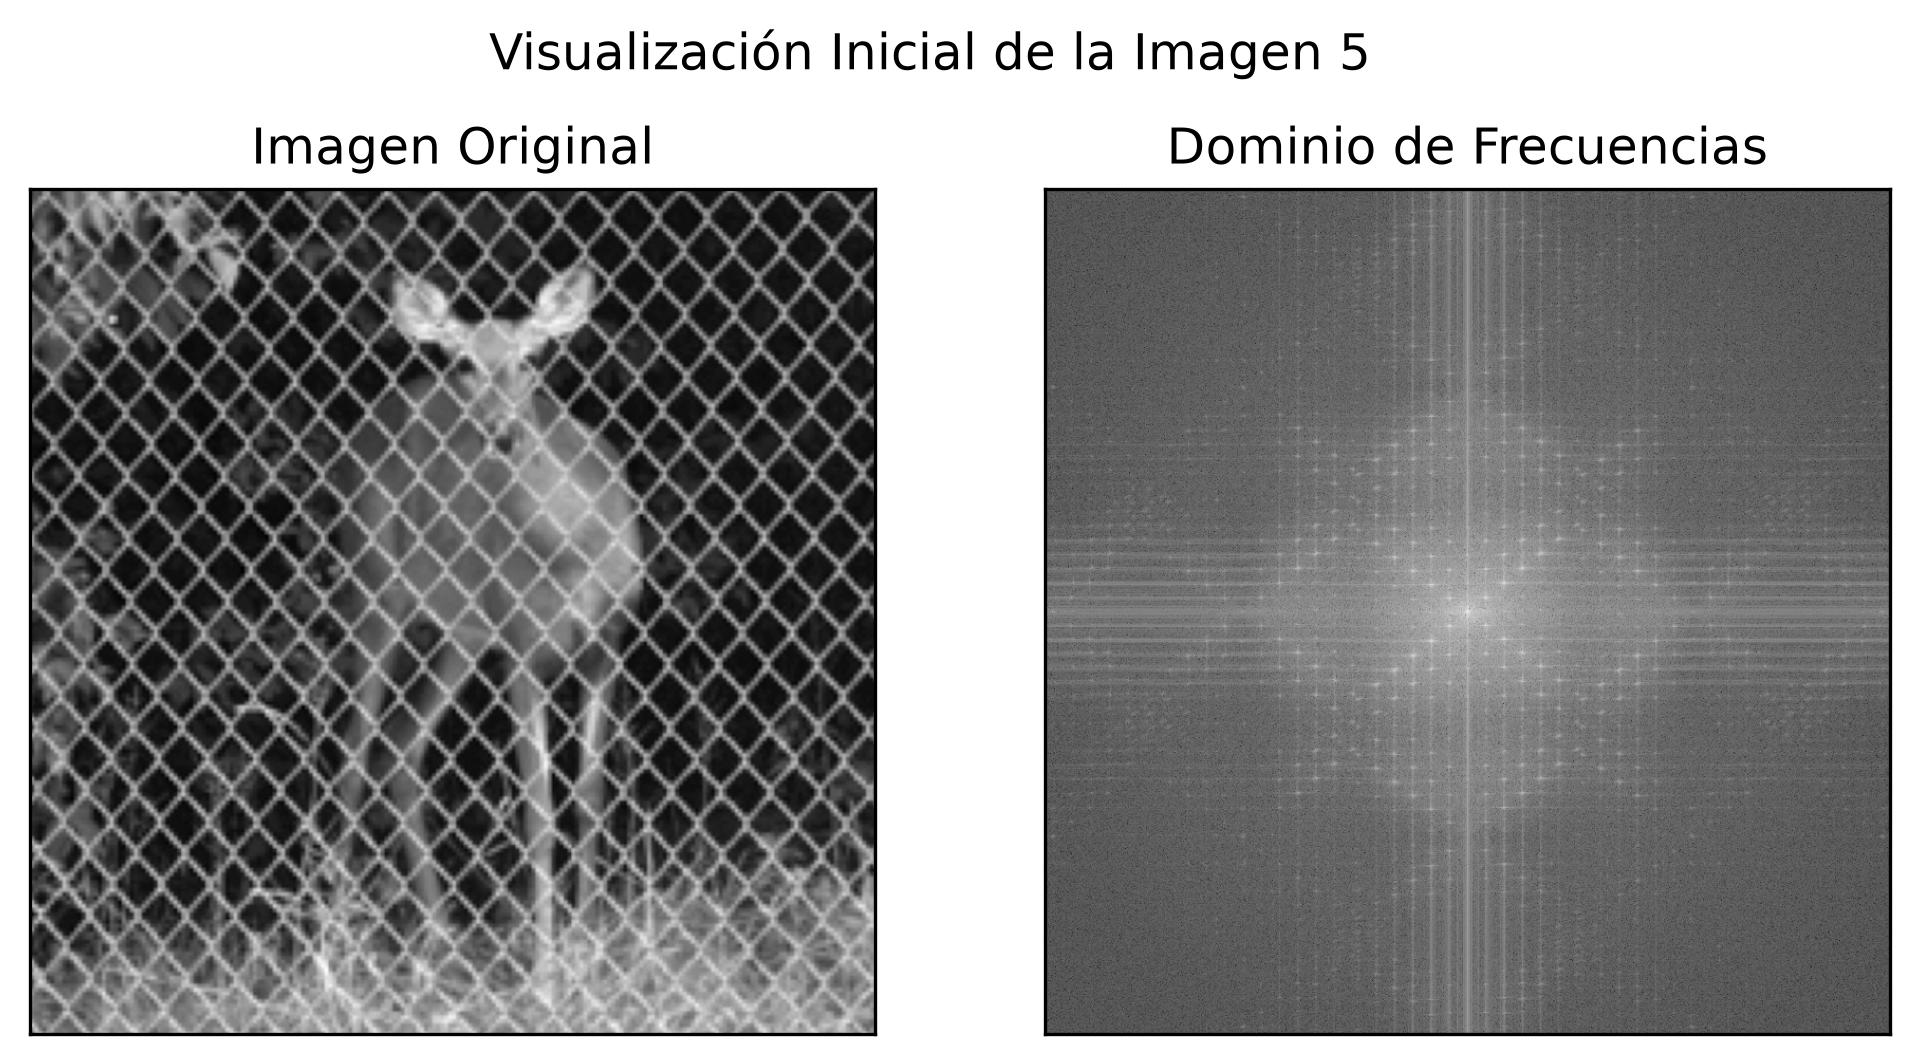
\includegraphics[width=0.65\textwidth]{../results/img_5_initial.jpg}
            \caption{Imagen 5 con ruido periódico.}
        \end{figure}

        \begin{figure}[H]
            \centering
            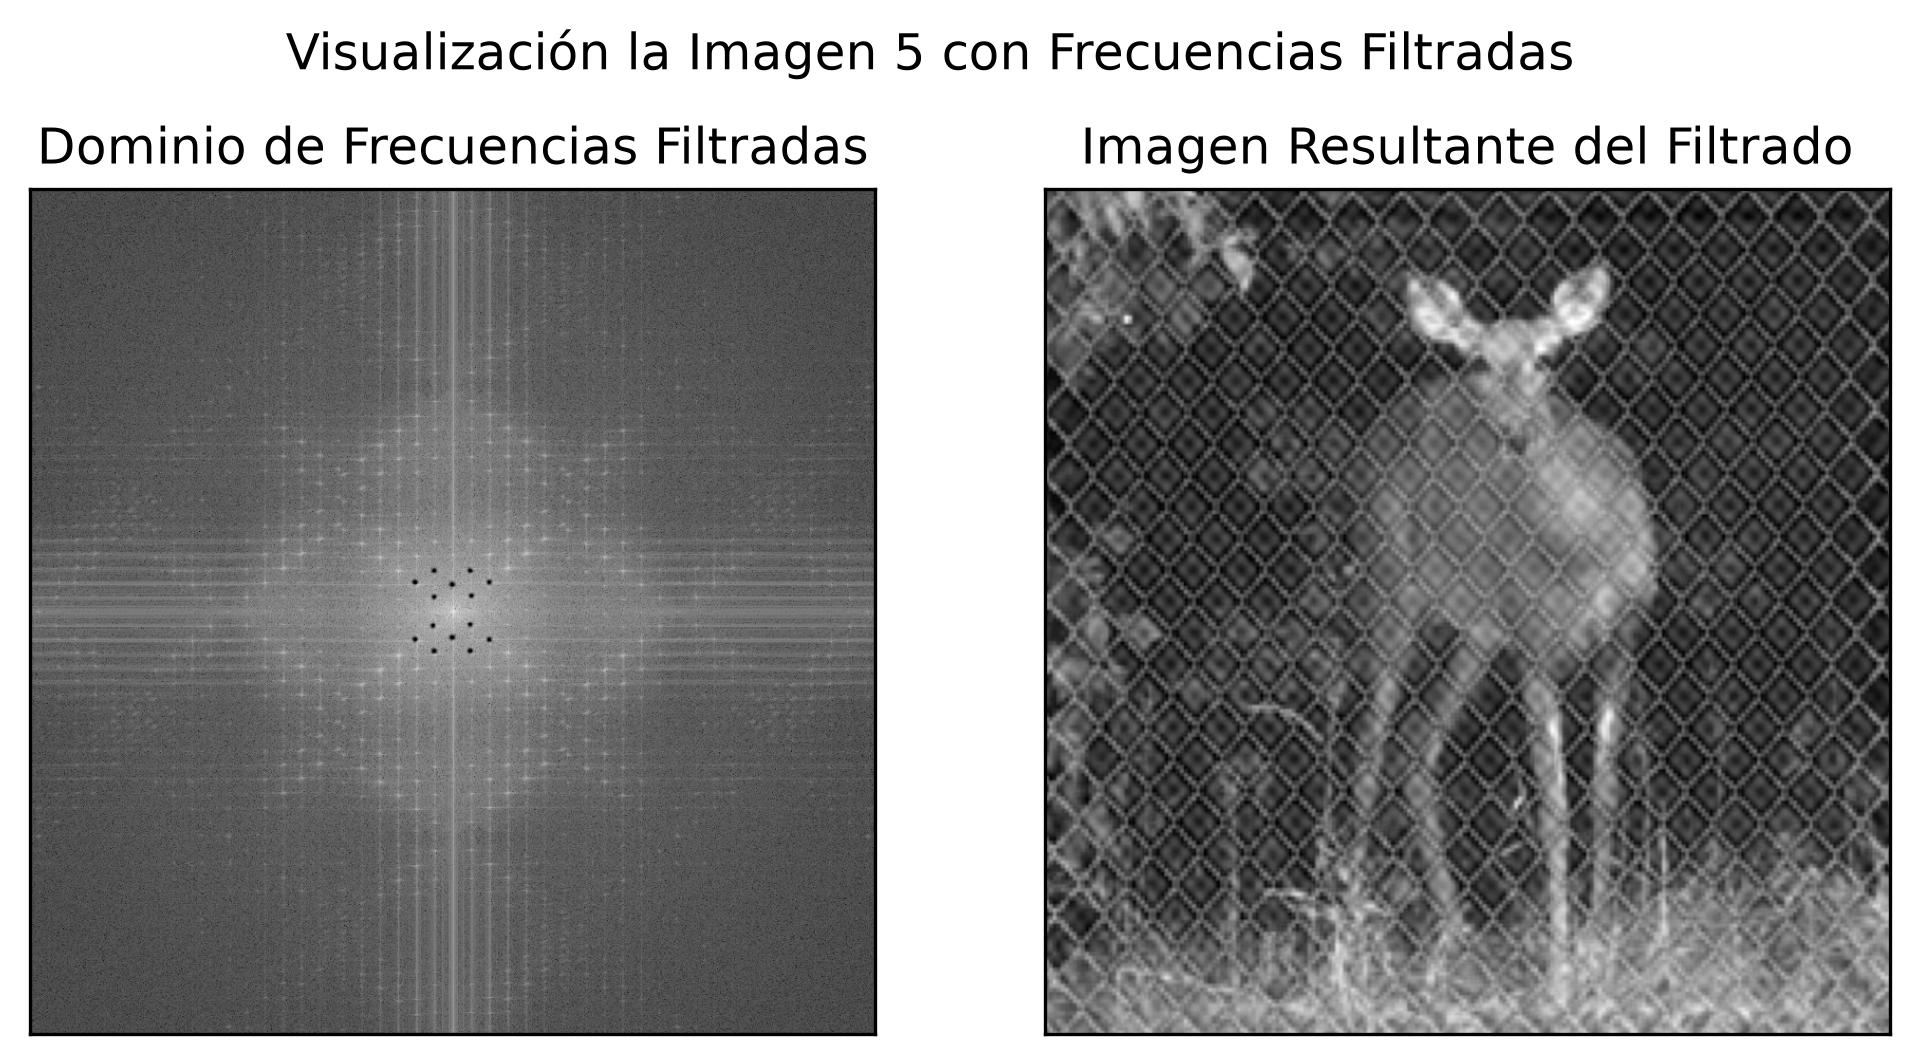
\includegraphics[width=0.65\textwidth]{../results/img_5_final.jpg}
            \caption{Imagen 5 después del filtrado de frecuencias.}
        \end{figure}
    